\chapter{Integration Tests} 
\label{chap:integration_tests}

This chapter aims to provide with an overview of the events the system goes
through to automatically scale a group of consumers, so as to achieve the
required parallelism to have the group consuming data from each partition at a
speed which is bigger or equal to their respective write speed. This involves
communication between all three components presented in Chapter
\ref{chap:consumer_group_autoscaler}, each playing a role in allowing the
problem to be modeled as a Bin Packing Problem.

\begin{figure}[htb!]
\centering
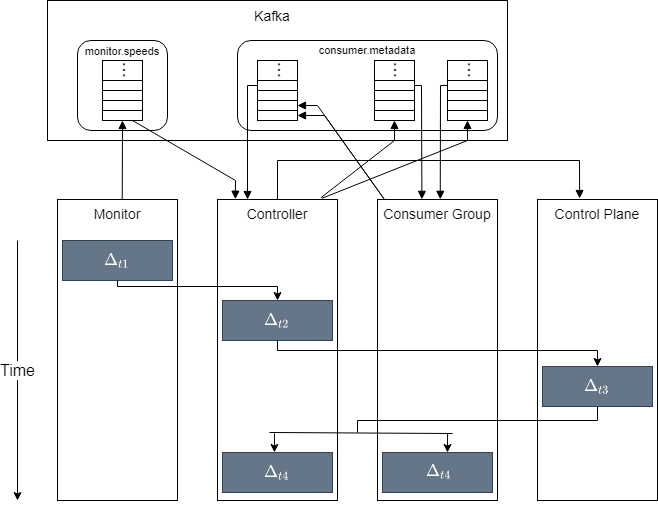
\includegraphics[width=\textwidth]{images/integration/Integration_diagram.png}
\caption{System sequence of events.}
\label{fig:step_event_sequence}
\end{figure}

Initially, a measurement has to be provided by the monitor process to then be
consulted by the controller ($\Delta_{t1}$). The controller then updates the
group's current state based on the new measurement, and proceeds to computing a
new group configuration using one of the heuristic algorithms presented in
Section \ref{subsub:modified_any_fit}.  Having calculated the new configuration,
the controller calculates the difference between the new and current
configuration, to determine the consumers it has to create, the ones it has to
delete, and the messages that have to be communicated to each consumer to reach
the intended state (Section \ref{sub:state_group_management}). This then leads
to the controller communicating with the Kubernetes control plane, to create the
new consumer resources ($\Delta_{t2}$). 

The controller then waits for the newly created deployments to be ready
($\Delta_{t3}$), followed by communicating with the consumer group to inform the
consumers of their change in state, which only terminates as
soon as all messages have been sent out to the respective consumers, and when every message
has been acknowledged back to the controller ($\Delta_{t4}$). This process is illustrated
by Figure \ref{fig:step_event_sequence}.


\section{Monitor Measurement Convergence Time ($\Delta_{t1}$)}
\label{c3sec:MonitorMeasurement}

To evaluate the monitor's response time, the data points were obtained by
feeding the system a step input, similar to what was done in Section
\ref{component:Monitor}, which is obtained by starting a producer that sends
data to one of the partitions the consumer group is consuming data from.

\begin{figure}[H]
\centering
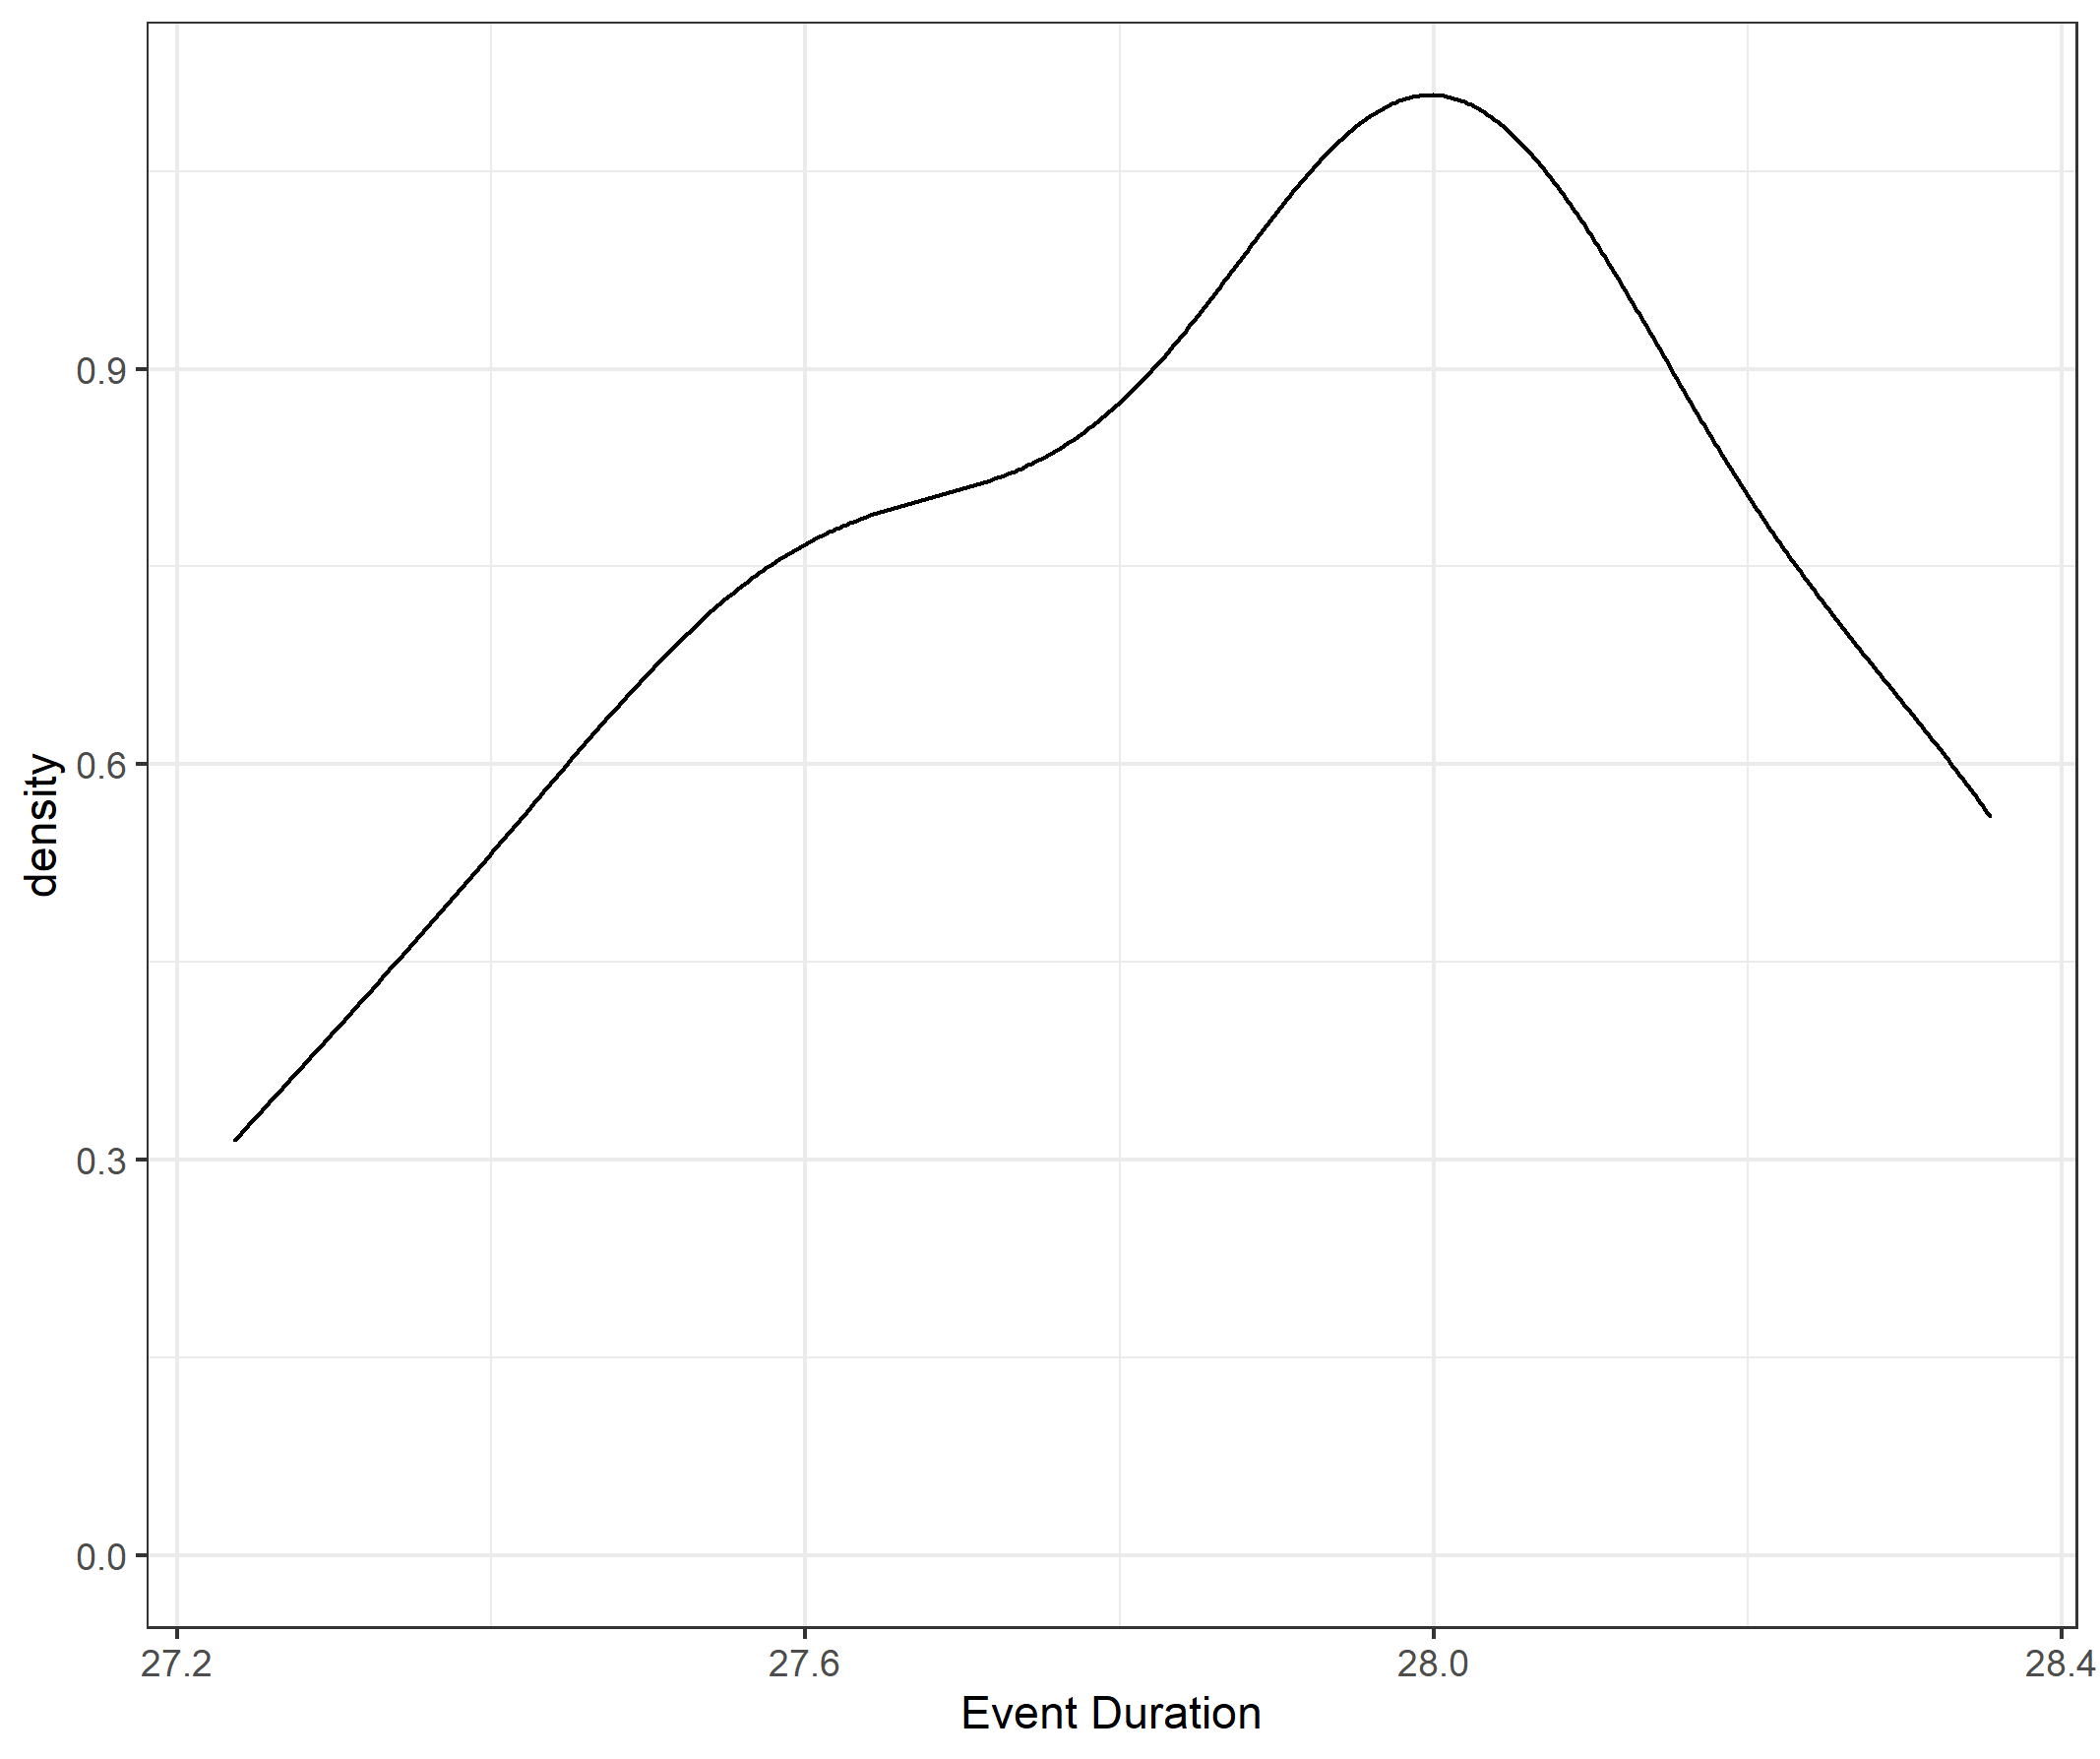
\includegraphics[width=0.6\textwidth]{images/integration/delta1.png}
\caption{
    Distribution of $\Delta_{t1}$ for 31 different step inputs.
}
\label{fig:controller_result_monitor}
\end{figure}

As such, this measure is the time it takes the monitor process to converge to
the real production rate, which, as can be verified in Figure
\ref{fig:controller_result_monitor}, takes no more than $30s$, similar to what
had been obtained in Figure \ref{fig:monitor_step}.

\section{Time to Trigger Scale-up ($\Delta_{t2}$)}

Measured as the time it takes the controller to compute the consumer group's new
assignment, computing the difference between the new and current states, and to
send an asynchronous request to the GKE cluster for every new consumer instance
to be created. To obtain the distribution for this metric, the system was tested
with the aforementioned step inputs and the randomly generated measurement
sequences used in Section \ref{c3subsub:testing}.

\begin{figure}[htb!]
\centering
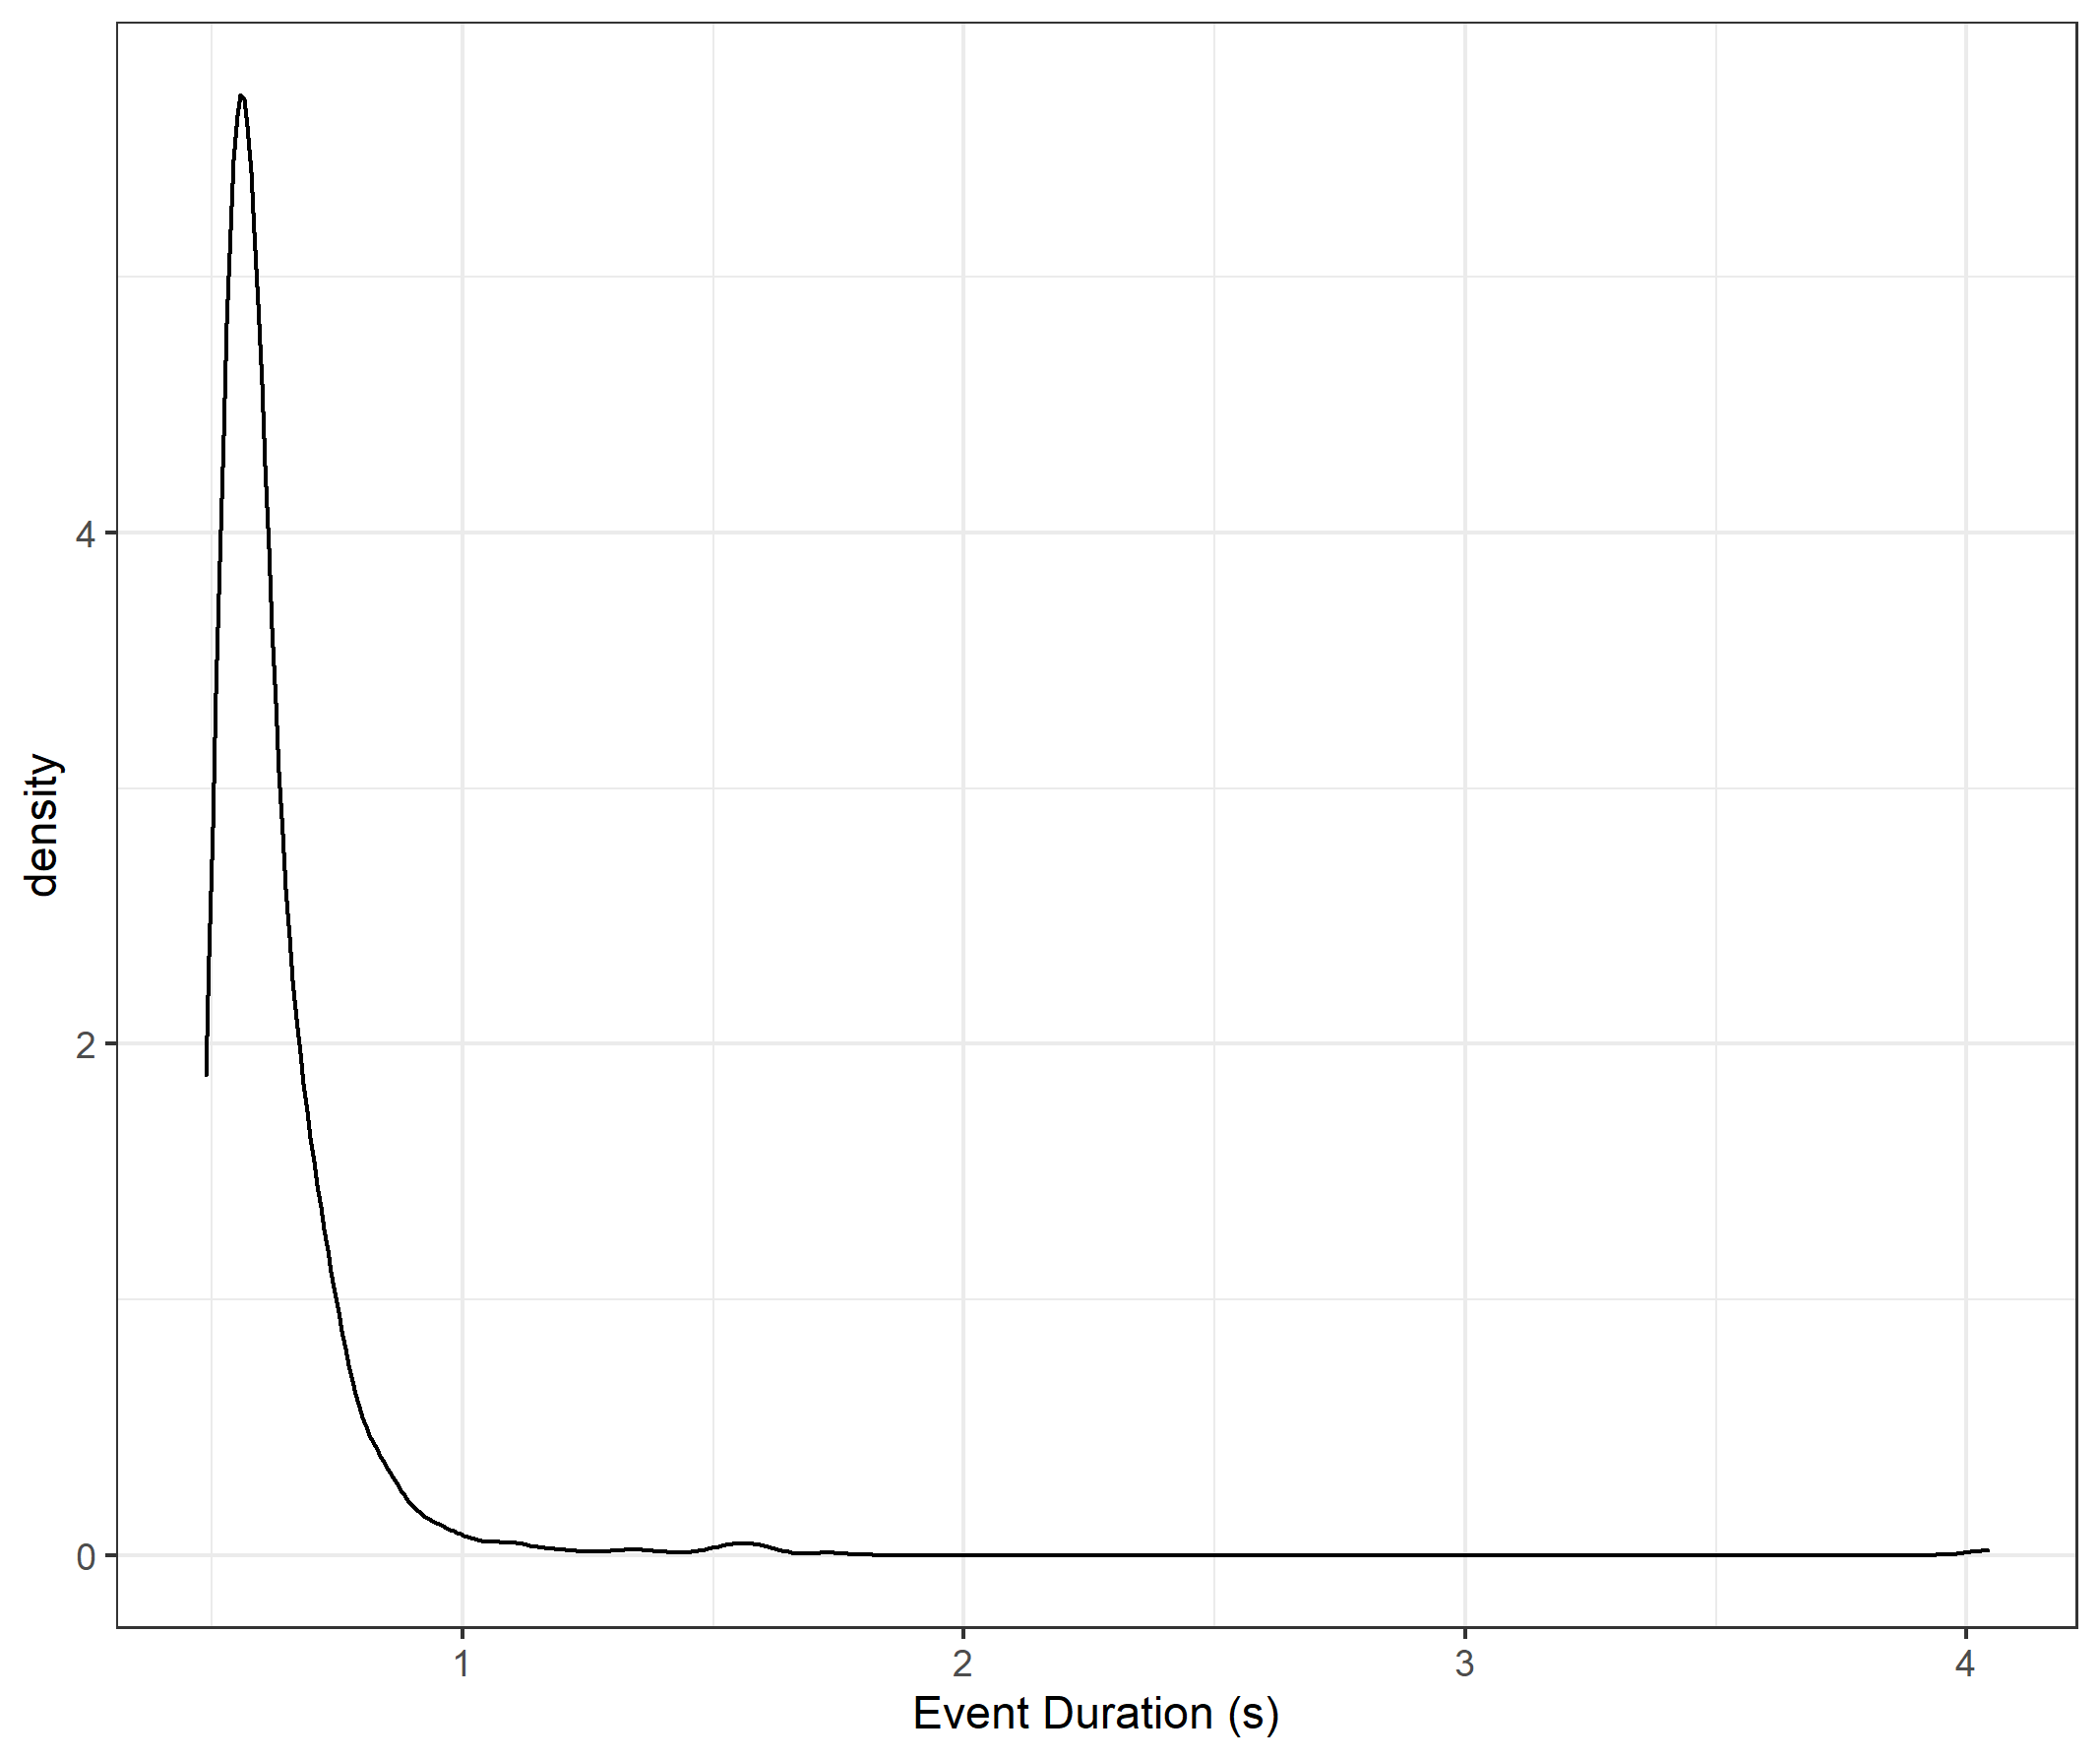
\includegraphics[width=0.6\textwidth]{images/integration/delta2.png}
\caption{
    Distribution of $\Delta_{t2}$ for 1345 observations.
}
\label{fig:controller_result_trigger}
\end{figure}

The time the controller takes with this procedure depends on the number of
partitions to distribute between the consumer group, the algorithm the
controller is executing to figure a new consumer group assignment, and the
number of new consumer instances it has to create in the GKE cluster.

For the tested input data, where there were at most 32 partitions to rebalance
and no more than 20 consumers to be created in a single interation, the event
consistently takes less than 1 second to be executed as shown in Figure
\ref{fig:controller_result_trigger}.

\section{Newly Created Deployments Ready ($\Delta_{t3}$)}

After making the asynchronous request to the GKE cluster, the control plane
schedules the pods to a node, and within the node starts the containers that are
to be executed.

\begin{figure}[htb!]
\centering
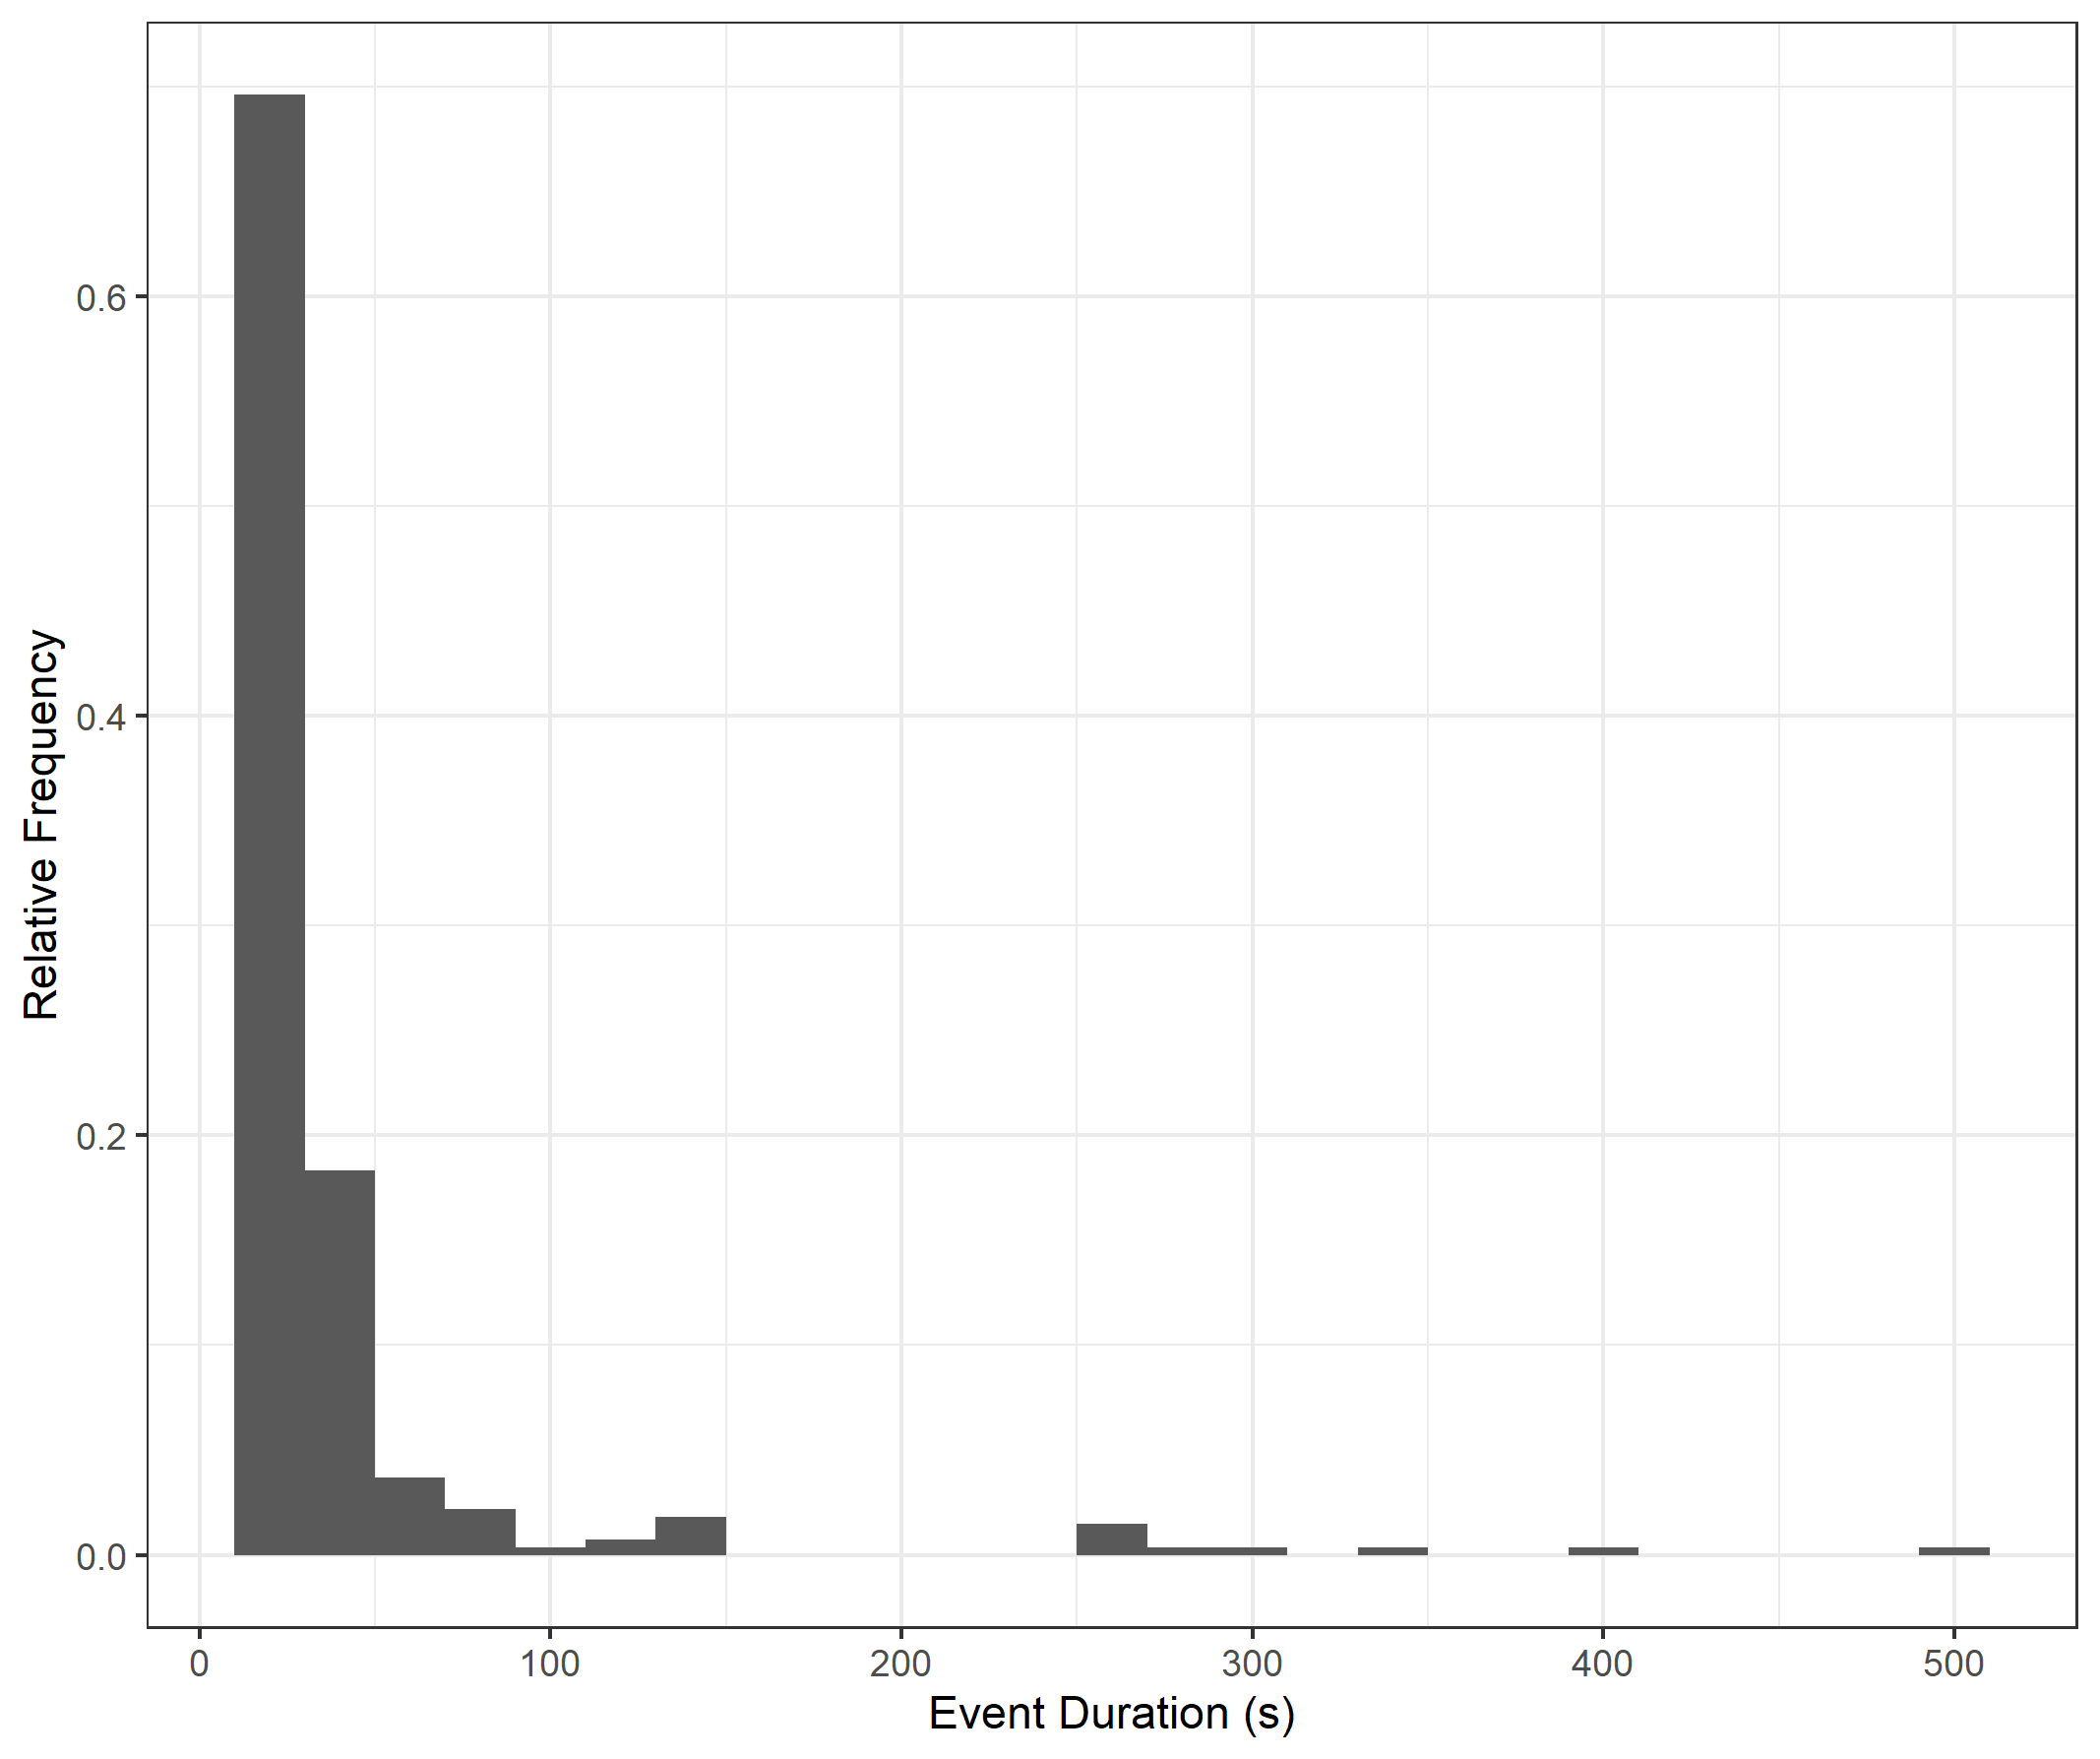
\includegraphics[width=0.6\textwidth]{images/integration/delta3.png}
\caption{
    Histogram of $\Delta_{t3}$ for 273 observations.
}
\label{fig:controller_result_kubernetes}
\end{figure}

After discarding the data points that didn't have the controller creating any
new consumer, there remain 273 data points, which show two clusters of data
points that are justified by two different scenarios when creating a new pod. 

The first, and most frequent (88\%), has the GKE cluster taking between $[10,
50]$ seconds to have a new consumer instance ready. This is usually the case when the
controller requests for the creation of new consumer instances and the
Kubernetes cluster has resources available to schedule the new consumer
instance. As such, the event's duration is related to the time it takes the
scheduled node(s) to download the image from the container registry, and to
start the containers.

The second group of data points, any time span greater than $50s$ (represents
12\% of the data points), occurs when the Kubernetes cluster does not have any
available resources. Here the actions the cluster undergoes are adding a new
node to the cluster, and only then scheduling the consumer instance into the new
available node. Due to the autoscaling feature of the GKE cluster, this is done
automatically but it is also more inconsistent, having data points taking up to
$500s$, although very sporadically.

Although there isn't much control over the time it takes the Kubernetes cluster
to schedule and start the pods, one variable that can be controlled is the size
of the image which has to be downloaded by the nodes that were assigned the
newly created consumer instances.

\section{Communicating Change in State ($\Delta_{t4}$)}

Each partition that the controller is monitoring can either be associated with a
start, stop, rebalance or a do nothing action. A start action refers to the case
where there is no consumer currently consuming data from the partition, and the
controller has assigned that partition to a consumer in its newly computed
consumer group state. The stop action occurs when the controller no longer wants
a consumer assigned to this partition therefore having no consumer fetching data
from this partition in the group's future state. Rebalancing happens when the
controller is changing the partition from being assigned from one consumer to
another. Lastly, as the name suggests, do nothing is when there are no actions to
be communicated for a partition. 

Since there is no concurrent read from the partition when the controller is
analyzing a start or a stop action, the controller can send this message as soon
as it enters this event, having to wait at most for one consumer cycle to receive
the acknowledgement by the consumer. 

When rebalancing, the controller has to first send out the stop command, wait
for a response, send out the start command, and wait for the response. Without
taking into account any processing and network delays, at worst, the controller
might have to wait for 2 consumer cycles to be able to rebalance a partition.

\begin{figure}[htb!]
\centering
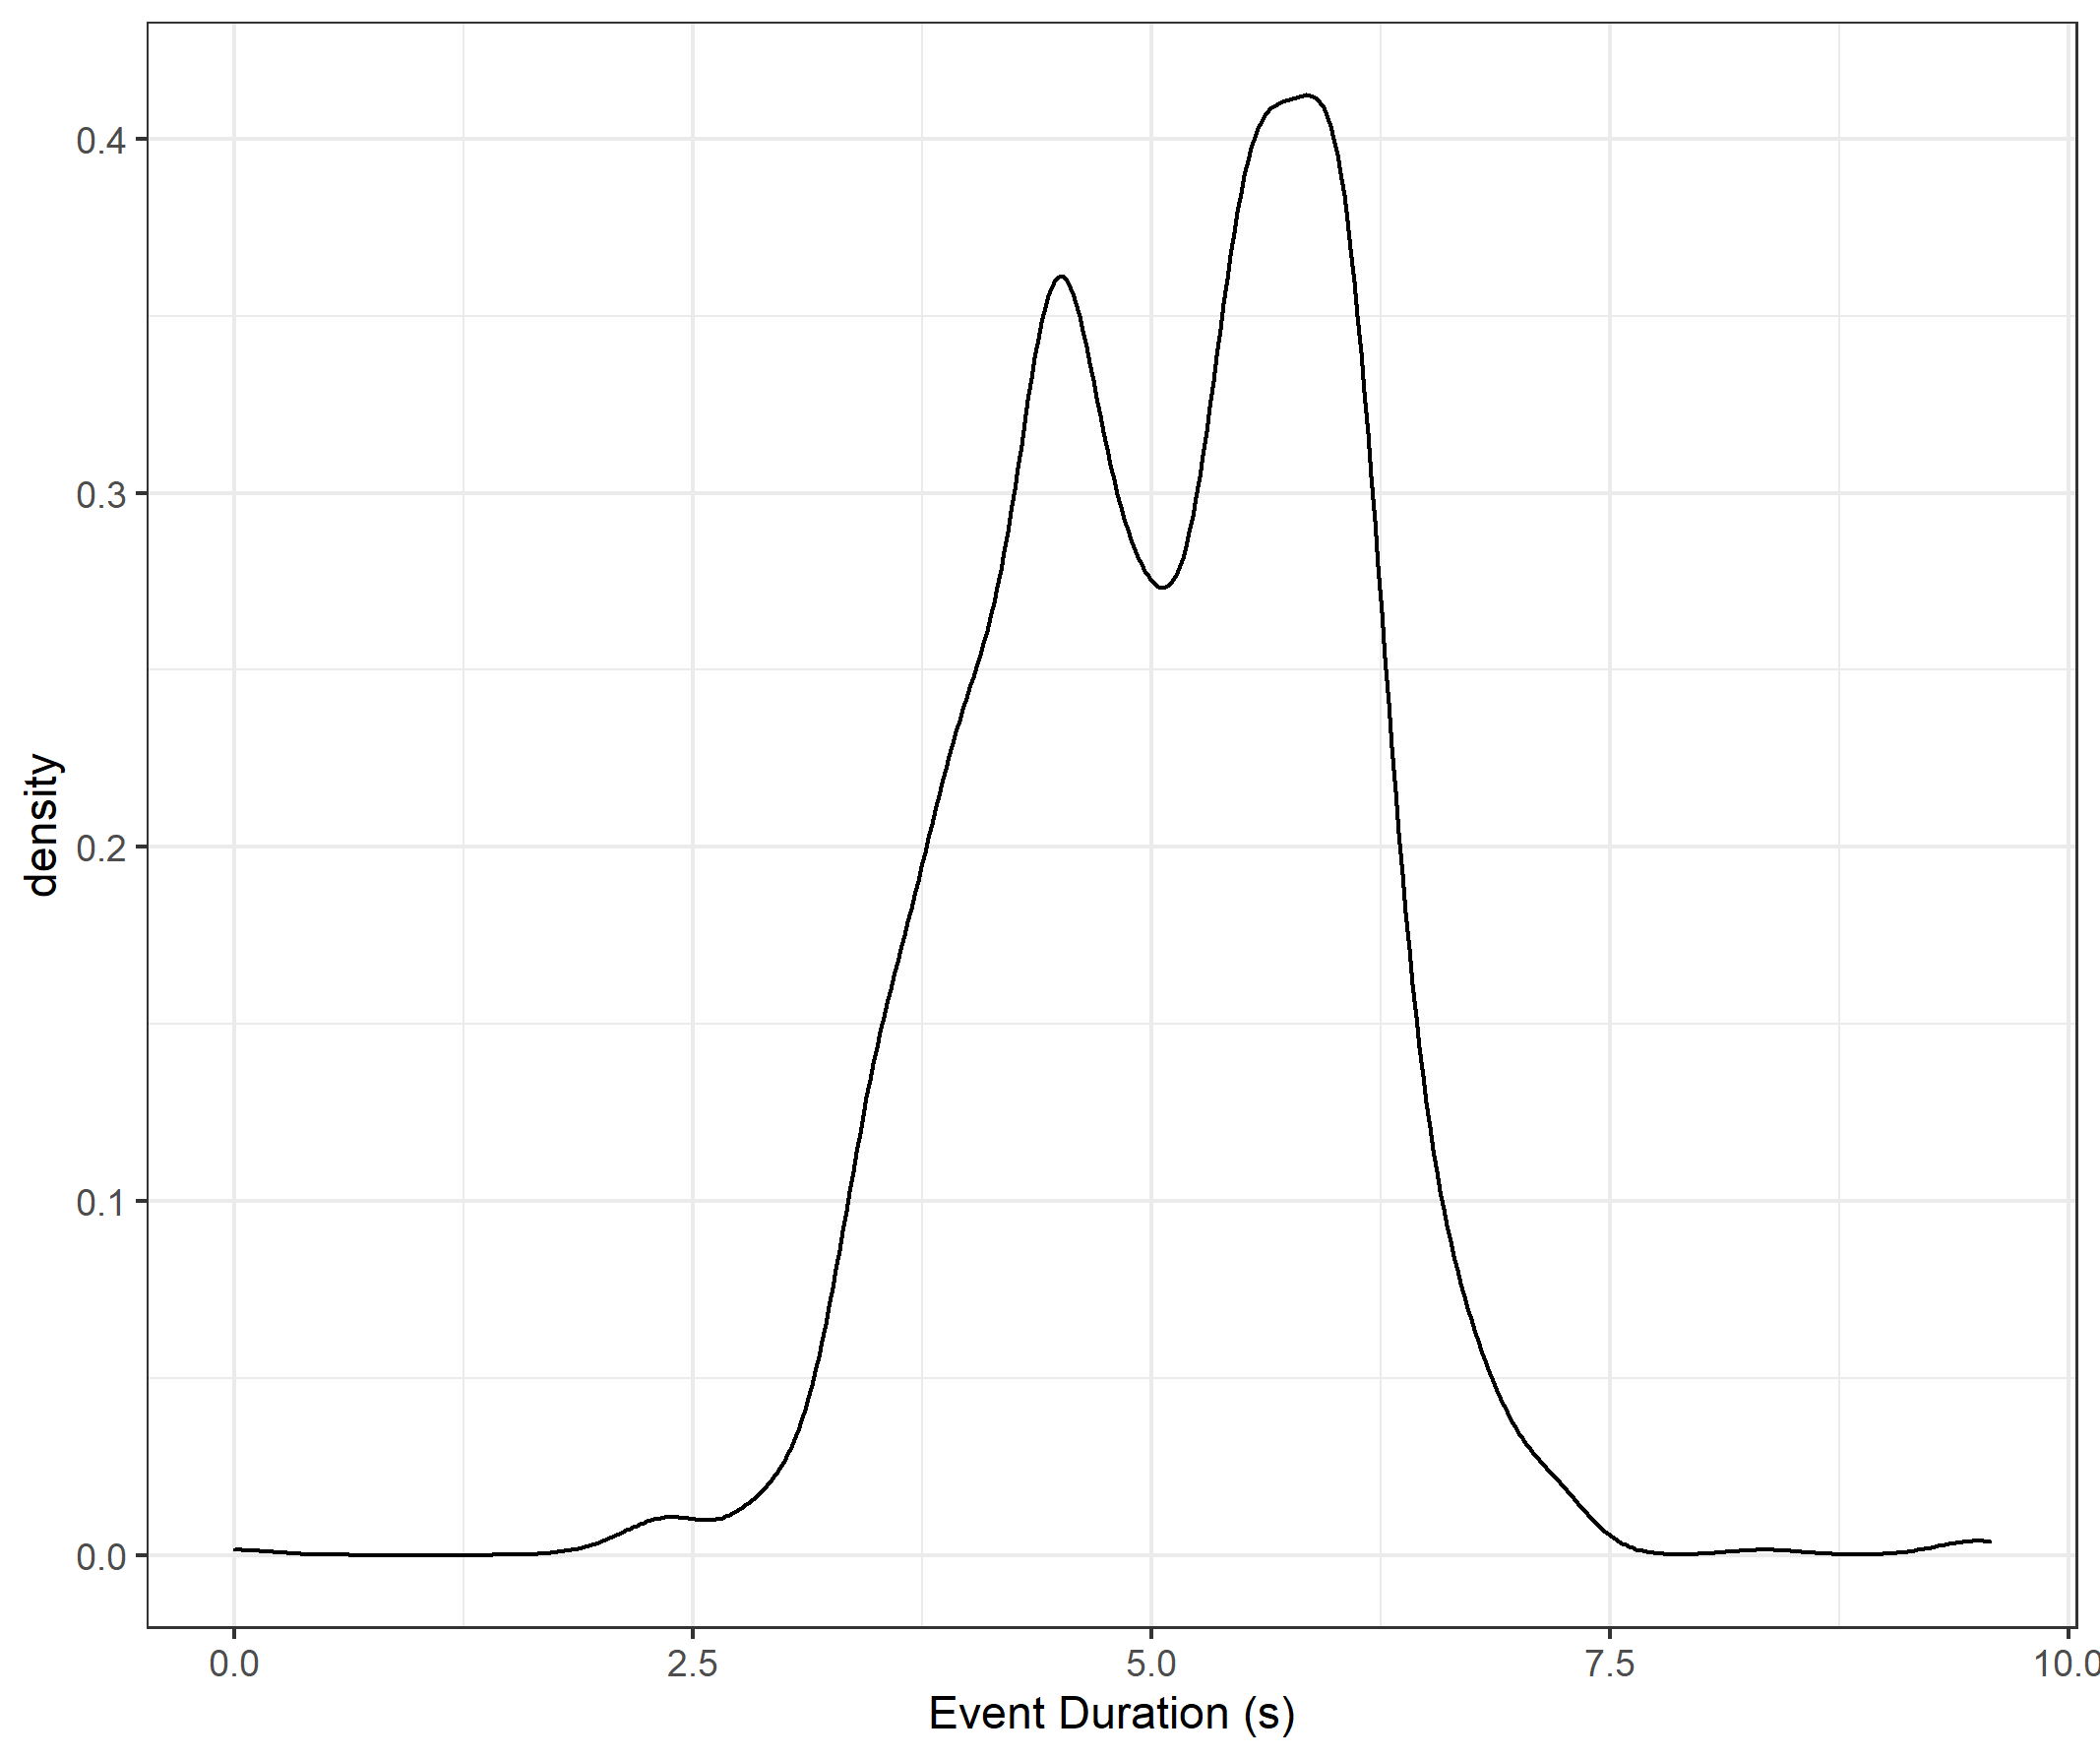
\includegraphics[width=0.6\textwidth]{images/integration/delta4.png}
\caption{
    Distribution of $\Delta_{t4}$ for 1331 observations.
}
\label{fig:controller_result_change_state}
\end{figure}

A consumer's insert cycle goes through the different phases mentioned in Section
\ref{component:consumer}, and only after performing it's tasks does it verify
the metadata queue to check if it has received any change in state command. For
this reason, between two metadata reads from the \lstinline{consumer.metadata}
topic, it takes the consumer one whole insert cycle. Having defined in Section
\ref{c3subsub:consumer_maximum_capacity} that the consumer gathers at most
$5Mbytes$ per cycle, and provided the results from Figure
\ref{fig:consumer_capacity}, which indicate the consumer has a data rate of
approximately $2Mbytes/s$, each consumer cycle can take approximately $2.5s$.
Since the controller has to wait for two consumer cycles, this would imply that
changing the group's state could take around 5 seconds, as can be seen in Figure
\ref{fig:controller_result_change_state}

It is also worth noting that the more consumers there are in the group, the
higher the probability that the controller has to wait 1 whole cycle after
sending out the stop command, and another whole cycle after a start command, as
the communication is performed with more consumers.

Although this analysis was performed for a single partition, without any loss of
generality and due to the fact that the controller sends out the change state
commands in batch, the time it takes the controller to change a consumer group's
state remains at 2 consumer cycles.

To vary the duration of this event, the consumer's cycle has to be altered using
the \lstinline{BATCH_BYTES} and \lstinline{WAIT_TIME_SECS} parameters, which in
turn have an effect on the time the consumer spends in a whole insert cycle.
